% ================================================================
% chapters/chapter1.tex --- RECONSTRUCTION (v2, remarques encadrant)
% ----------------------------------------------------------------
% Base : ma précédente reconstruction (Start Beyond + Fondements
% pédagogiques + Blender 5.1 déjà fusionnés), + toutes les remarques
% de RemarquesChap1.pdf qui ne dépendent PAS d'une info externe.
%
% APPLIQUÉ ICI :
%   - Intro sentences ajoutées : 1.6 (Étude existant), 1.6.1 (LMS),
%     1.6.2 (VR existantes), 1.8/1.8.1/1.8.2/1.8.3 (Environnement)
%   - 1.5.1.1 TalentLMS fusionné dans 1.6.1 (plus de sous-titre,
%     un seul exemple)
%   - "Positionnement de TynassIt" fusionné dans "Etude comparative"
%     (plus de sous-titre séparé)
%   - "Fondements pédagogiques" déplacé en section 1.5 propre,
%     sortie de "Étude de l'existant"
%   - "Tableau comparatif" renommé "Etude comparative"
%   - Note "Start Beyond n'apparaît pas dans le tableau..." supprimée
%   - Fonctionnalités ajouté pour ClassVR et Meta Quest for Business
%   - "Limite" -> "Limites" (BCG, Accenture, ClassVR, Start Beyond)
%   - "Sa mission" -> "Sa devise"
%   - "application VR Unity~6" -> "application VR" (Objectifs)
%   - "avec les encadrants" -> "avec le Product Owner" (1.7.2)
%
% VOLONTAIREMENT PAS TOUCHÉ (en attente) :
%   - 1.4.1 Problématique : toujours vide
%   - 1.2 Cadre général : "Pfe licence ?, CM ?" pas répondu --- la
%     phrase actuelle reste, à préciser toi-même
%   - Rôles Scrum (1.7.3 après renumérotation) : attend le nom du PO
%     côté Indigo
%   - Planning global / tableau épics-sprints (1.7.4) : attend une
%     refonte méthodologique, pas juste un mot à changer
%
% PAS DANS CE FICHIER (vit ailleurs) :
%   - Ajout de "XR" dans la Liste des abréviations (autre fichier)
%   - Bug de mise en page (tableau abréviations qui chevauche "xiii")
% ================================================================

\chapter{Contexte général}

\section{Introduction}

Ce chapitre présente le contexte général du projet. Nous introduisons l'organisme d'accueil,
le cadre du projet, la problématique retenue et ses objectifs. Une étude de l'existant permet
de positionner \tynassit{} par rapport aux solutions disponibles. Nous détaillons ensuite
la méthodologie adoptée, le planning du projet et l'environnement de développement.

\section{Cadre général du projet}

Ce projet s'inscrit dans le cadre du Projet de Fin d'Études (PFE) d'\textbf{ingénieur},
spécialité \textbf{Image Numérique et Réalité Virtuelle}, d'une durée de
\textbf{six mois}, dont \textbf{quatre mois} consacrés au développement effectif.
Il est réalisé au sein de \textbf{Tynass IT}, une entreprise tunisienne spécialisée dans le
développement d'expériences immersives en Réalité Étendue (XR).

\section{Organisme d'accueil --- Tynass IT}

Ce projet a été réalisé au sein de Tynass IT. Cette section présente l'entreprise
d'accueil et les projets qu'elle a menés dans le domaine des expériences immersives.

\subsection{Présentation de Tynass IT}

Tynass IT dont le logo est représenté sur la figure~\ref{fig:logo_tynass} est une entreprise tunisienne fondée en \textbf{2020}, spécialisée dans le
développement d'expériences immersives en XR (Réalité Virtuelle, Augmentée et Mixte).
Sa devise~: \og~\textit{Elevating Ideas, Creating Experiences}~\fg, traduit son engagement
à transformer des idées complexes en expériences numériques mémorables.

\begin{figure}[H]
  \centering
  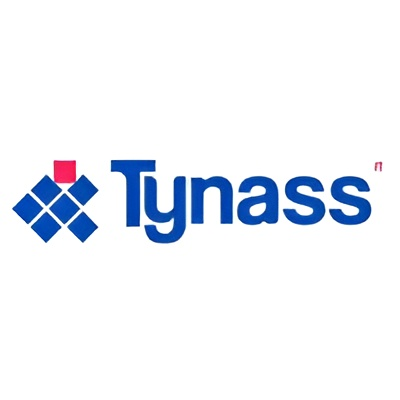
\includegraphics[width=0.35\textwidth]{../images/logo_tynass.jpg}
  \caption{Logo de Tynass IT}
  \label{fig:logo_tynass}
\end{figure}

Tynass accompagne des institutions culturelles, des entreprises et des organismes
publics dans leur transition vers des expériences numériques immersives, en exploitant
les technologies les plus avancées du marché XR.

\subsection{Projets réalisés}

Avant ce PFE, Tynass a développé plusieurs projets XR remarquables~:

\begin{itemize}
  \item \textbf{Immersive Tunisia}~: une expérience de Réalité Mixte sur Meta Quest~3,
    combinant VR, AR et contenu web pour faire revivre le patrimoine tunisien. Les utilisateurs
    explorent des modèles 3D de monuments historiques avec des portails interactifs gamifiés.

  \item \textbf{Farhat Hached VR/Web Experience}~: une galerie VR immersive retraçant la vie
    du syndicaliste Farhat Hached, avec une collection de photos rares et de documents d'archive.

  \item \textbf{Habib Bourgiba VR Experience}~: une galerie VR mettant en lumière la vie de
    Habib Bourgiba, avec une recréation 3D de l'un de ses discours historiques.

  \item \textbf{Tynass Trips}~: une application mobile de guidage touristique immersif avec
    narration audio multilingue, comptant plus de \textbf{1500 utilisateurs} sur iOS et Android.
\end{itemize}

\section{Présentation du projet}

Apres avoir presente l'organisation d'accueil, cette section expose la problématique à l'origine du projet, puis les objectifs fixés
pour y répondre.

\subsection{Problématique}

De nombreuses entreprises consacrent un temps et des ressources considérables à la
formation de leurs employés sur des procédures, des tâches ou des protocoles qui
nécessitent une réelle expérience pratique pour être maîtrisés, ou dont l'apprentissage
par les méthodes traditionnelles (formations présentielles, manuels, tutorat) s'avère
particulièrement long. Ce temps de formation représente un coût direct~: mobilisation
des formateurs et des managers, ralentissement de la montée en autonomie des nouveaux
employés, et résultats d'apprentissage difficiles à standardiser ou à vérifier
objectivement.

La réalité virtuelle constitue une réponse pertinente à ce type de problématique,
comme le confirment les données évoquées en introduction~: son caractère immersif et
expérientiel la rend particulièrement adaptée à l'apprentissage de compétences
procédurales et situées, là où les supports classiques peinent à reproduire une
véritable mise en situation.

\begin{notebox}
  \textbf{Problématique}~: comment concevoir et developper une plateforme de formation immersive
  capable de réduire le temps de montée en autonomie sur des procédures complexes,
  tout en offrant un moyen mesurable d'en vérifier les acquis~?
\end{notebox}

\subsection{Objectifs}

Pour valider cette approche sur un cas réel, nous avons choisi de développer un
premier module de formation en partenariat avec \textbf{Indigo Company}, leader
tunisien du prêt-à-porter regroupant treize enseignes aux identités et procédures
propres. Chez Indigo, l'intégration d'un nouvel employé repose aujourd'hui
principalement sur un accueil RH ponctuel suivi d'un accompagnement de proximité avec
le N\texttt{+}1, sur une période de deux semaines en moyenne~--- une approche où le
temps consacré dépend directement de la disponibilité du manager, et où aucun
mécanisme systématique ne permet de vérifier qu'un nouvel employé maîtrise
effectivement les règles et procédures essentielles avant d'être considéré comme
autonome.

En réponse à cette problématique, et à travers ce cas d'usage, \tynassit{} vise à~:

\begin{itemize}
  \item Concevoir et développer un \textbf{backend REST sécurisé} gérant les entreprises
    clientes, les formations VR et le suivi des sessions.
  \item Développer un \textbf{dashboard web Admin} permettant aux équipes Tynass de gérer
    les entreprises, les formations et les casques Meta Quest~3.
  \item Développer un \textbf{dashboard web Company} permettant aux entreprises clientes
    de gérer leurs employés et de consulter leurs performances.
  \item Développer une \textbf{application VR} offrant aux employés une expérience
    de formation immersive avec envoi automatique des résultats.
  \item Réaliser le premier module de formation pour \textbf{Indigo Company}~:
    simulation d'intégration des nouveaux employés.
\end{itemize}

\section{Fondements pédagogiques du choix de la VR}

Au-delà des indicateurs sectoriels déjà cités en introduction~\cite{pwc2020}, le choix
de la VR comme support pédagogique s'appuie sur deux corpus théoriques distincts de la
littérature académique.

\paragraph{Double codage de l'information.}
La théorie du double codage~\cite{paivio1971,clarkpaivio1991} établit que l'information
encodée simultanément par le canal verbal et le canal visuel bénéficie de deux traces
mnésiques indépendantes, augmentant significativement les chances de rappel par rapport
à un encodage mono-canal. Ce principe justifie la combinaison, dans \tynassit{}, de la
narration audio, du texte informatif et de la représentation visuelle~3D des lieux et
procédures, plutôt qu'un support uniquement textuel ou uniquement oral.

\paragraph{Apprentissage expérientiel et présence immersive.}
Au-delà du simple visuel, la spécificité de la VR tient à l'immersion et à
l'expérience à la première personne. Une revue systématique de l'usage de la VR en
éducation~\cite{radianti2020} et le modèle des \textit{learning affordances} des
environnements 3D~\cite{dalgarnolee2010} convergent~: le sentiment de présence en
environnement virtuel immersif améliore la mémorisation spatiale, l'engagement et la
rétention de connaissances, en particulier pour des tâches procédurales et
situées~--- exactement le cas d'usage de l'intégration de nouveaux employés visé par
la simulation d'intégration d'Indigo.

\begin{notebox}
  Il convient de nuancer~: l'efficacité de la VR n'est pas uniforme selon le type de
  tâche. Elle est particulièrement démontrée pour les compétences procédurales et
  situées~--- se repérer dans un lieu, suivre une procédure, réagir à une
  situation~--- et moins systématiquement supérieure aux supports électroniques
  classiques pour l'acquisition de connaissances purement déclaratives. C'est ce
  périmètre précis (repérage, procédures, mise en situation) que cible cette
  simulation d'intégration, plutôt qu'une prétention à remplacer tout support de formation.
\end{notebox}

\section{Étude de l'existant}

Cette section présente les principales solutions de formation existantes sur le marché,
qu'il s'agisse de plateformes LMS traditionnelles ou de solutions immersives en VR, afin
de positionner \tynassit{} par rapport à l'offre actuelle.

\subsection{Solutions LMS traditionnelles}

Un LMS (\textit{Learning Management System}) est une plateforme logicielle dédiée à la
gestion, la diffusion et le suivi de contenus de formation en ligne.

TalentLMS~\cite{talentlms2026} est la plateforme LMS cloud \#1 mondiale, utilisée par plus
de \textbf{70 000 équipes} à travers le monde (dont Google, Amazon, Meta, PwC).

\begin{itemize}
  \item \textbf{Fonctionnalités}~: création de cours en ligne, suivi des progrès, certifications,
    onboarding, application mobile, intégrations (Slack, Zoom, SCORM).
  \item \textbf{Certifications}~: ISO/IEC 27001:2022, ISO 9001:2015, conforme RGPD.
  \item \textbf{Limites pour notre cas}~: formation uniquement en 2D (vidéos, quiz en ligne),
    pas de simulation immersive pas d'adaptation au contexte terrain métier.
\end{itemize}

\subsection{Solutions VR existantes}

Plusieurs grandes entreprises et plateformes ont développé des solutions de formation en
réalité virtuelle, à des échelles et avec des objectifs variés.

\subsubsection{BCG Universe}

Boston Consulting Group a déployé \textbf{BCG Universe}~\cite{bcg2024} en 2024, un programme
d'onboarding en VR destiné à ses nouvelles recrues mondiales.

\begin{itemize}
  \item \textbf{Résultats}~: 100\% de satisfaction des participants, Gold Award
    Brandon Hall Excellence Awards 2024.
  \item \textbf{Limites}~: solution interne, budget de plusieurs millions de dollars,
    non accessible aux PME.
\end{itemize}

\subsubsection{Accenture Nth Floor}

Accenture a développé \textbf{Nth Floor}~\cite{accenture2025}, un environnement métaverse
pour l'intégration de ses nouvelles recrues.

\begin{itemize}
  \item \textbf{Fonctionnalités}~: visite virtuelle des bureaux, présentation des équipes,
    collaboration immersive.
  \item \textbf{Limites}~: solution propriétaire non commercialisée, réservée en interne.
\end{itemize}

\subsubsection{ClassVR}

ClassVR est une plateforme VR dédiée à l'éducation, proposant des casques spécifiques
pour les établissements scolaires.

\begin{itemize}
  \item \textbf{Fonctionnalités}~: contenus pédagogiques immersifs et casques VR dédiés,
    conçus spécifiquement pour un usage en salle de classe.
  \item \textbf{Limites}~: orientée enfants et adolescents, pas adaptée à la formation
    professionnelle adulte en entreprise.
\end{itemize}

\subsubsection{Meta Quest for Business}

Meta Quest for Business était un bundle enterprise combinant casques Quest et outils de
gestion d'entreprise.

\begin{itemize}
  \item \textbf{Fonctionnalités}~: bundle combinant casques Meta Quest et outils de gestion
    d'entreprise (déploiement, gestion des appareils, support).
  \item \textbf{Arrêt}~: Meta a annoncé l'arrêt de ce programme en \textbf{février 2026},
    citant une demande insuffisante et un marché pas encore assez mature.
\end{itemize}

\subsubsection{Start Beyond}

Start Beyond~\cite{startbeyond2026} est une entreprise australienne fondée en 2015,
spécialisée dans la conception de contenus VR/AR sur mesure pour l'entreprise et
l'éducation, via son studio de production et sa plateforme \textbf{Oncio}.

\begin{itemize}
  \item \textbf{Fonctionnalités}~: formations immersives à la demande (onboarding,
    certification, sécurité, compétences comportementales), déployées pour des
    clients tels que St John Ambulance ou Qantas.
  \item \textbf{Limites}~: prestataire généraliste multi-secteurs~--- chaque
    simulation est développée sur mesure pour un client donné, sans plateforme
    de gestion exposée à l'entreprise cliente~; les indicateurs de performance
    communiqués (ex.\ « 2x faster training times », « 97\% increased confidence »)
    relèvent de communications commerciales et ne sont pas appuyés par une
    méthodologie publique vérifiable.
\end{itemize}

\subsection{Étude comparative}

Le tableau~\ref{tab:comparatif} présente une synthèse comparative des solutions existantes
par rapport à \tynassit{}.

\begin{table}[H]
  \centering
  \begin{tabularx}{\textwidth}{Xccccc}
    \toprule
    \textbf{Critère} & \textbf{TalentLMS} & \textbf{BCG} & \textbf{ClassVR}
                     & \textbf{Meta QB} & \textbf{\tynassit{}} \\
    \midrule
    B2B               & \checkmark & \checkmark & $\times$   & \checkmark & \checkmark \\
    VR immersive      & $\times$   & \checkmark & \checkmark & $\times$   & \checkmark \\
    Plateforme gestion& \checkmark & $\times$   & \checkmark & \checkmark & \checkmark \\
    Suivi sessions    & \checkmark & $\times$   & $\times$   & $\times$   & \checkmark \\
    Meta Quest 3      & $\times$   & $\times$   & $\times$   & $\times$   & \checkmark \\
    PME Tunisie       & $\times$   & $\times$   & $\times$   & $\times$   & \checkmark \\
    \bottomrule
  \end{tabularx}
  \caption{Synthèse comparative des solutions existantes}
  \label{tab:comparatif}
\end{table}

L'analyse des solutions existantes révèle un vide significatif~: aucune solution ne combine
simultanément l'immersion VR sur Meta Quest~3, une plateforme de gestion B2B intégrée et
une accessibilité adaptée aux entreprises tunisiennes. \tynassit{} se positionne précisément
dans cet espace, en offrant une alternative abordable aux solutions VR enterprise coûteuses
(BCG, Accenture), tout en dépassant les capacités des LMS classiques (TalentLMS) par
l'immersion et l'interactivité.

\section{Méthodologie de développement}

Le déroulement du projet repose sur une méthodologie de travail structurée. Cette section
compare les grandes familles de méthodologies, justifie l'approche retenue, décrit
l'organisation du travail et présente le planning global.

\subsection{Comparaison des méthodologies}

Le choix d'une méthodologie de gestion de projet constitue une décision structurante pour
le déroulement du développement. Le tableau~\ref{tab:methodo} présente une comparaison entre
les approches traditionnelles et agiles~\cite{agile2020}.

\begin{table}[H]
  \centering
  \begin{tabularx}{\textwidth}{lXX}
    \toprule
    \textbf{Critère} & \textbf{Traditionnel (Waterfall)} & \textbf{Agile (itératif / incrémental)} \\
    \midrule
    Cycle de développement & Séquentiel et linéaire & Itératif et incrémental \\
    Gestion des besoins & Définis en amont & Évolutifs à chaque itération \\
    Flexibilité & Faible & Forte \\
    Livraisons & Une seule livraison finale & Incréments fréquents \\
    Adaptation & Difficile & Naturelle \\
    \bottomrule
  \end{tabularx}
  \caption{Comparaison des méthodologies traditionnelles et agiles}
  \label{tab:methodo}
\end{table}

\subsection{Choix de l'approche itérative et incrémentale}

La nature de ce projet~--- évolutif, avec un client pilote (Indigo Company) dont les
besoins peuvent évoluer, et mené par un développeur unique~--- appelle une approche
flexible. Une démarche \textbf{itérative et incrémentale}, inspirée des principes agiles,
a été retenue pour les raisons suivantes~:

\begin{itemize}
  \item Des itérations courtes permettant de valider régulièrement l'avancement.
  \item Une adaptation facile aux changements de priorités (règlement intérieur Indigo, retours terrain).
  \item Des livraisons incrémentales permettant de tester chaque composante sur le casque physique.
  \item Un backlog produit structurant clairement les priorités via la méthode MoSCoW.
\end{itemize}

\subsection{Organisation du travail}

Le projet a été mené par un \textbf{développeur unique}~: nous avons assuré la conception, le
développement, les tests et la livraison de chaque incrément. Nous nous sommes appuyés
sur un encadrement à trois niveaux~: un \textbf{encadrement technique} assuré par le
Lead Tech de Tynass~IT (choix d'architecture, revue technique, déblocage), un
\textbf{encadrement stratégique} assuré par la direction de l'entreprise (vision
produit, priorités), et un \textbf{encadrement académique} assuré par l'enseignant
référent.


\subsection{Planning global du projet}

\begin{figure}[H]
  \centering
  \resizebox{\textwidth}{!}{%
  \begin{ganttchart}[
    hgrid, vgrid,
    bar/.append style={fill=coverblue!70},
    bar height=0.5,
    group/.append style={fill=coverblue},
    group peaks tip position=0,
    title/.append style={fill=coverblue!15},
    title label font=\small\bfseries,
    bar label font=\small,
    group label font=\small\bfseries,
    milestone/.append style={fill=covergray}
  ]{1}{24}
    \ganttset{calendar week text = S\currentweek{}}
    \gantttitle{Mars}{4} \gantttitle{Avril}{4} \gantttitle{Mai}{4}
    \gantttitle{Juin}{4} \gantttitle{Juillet}{4} \gantttitle{Août}{4} \\

        \ganttgroup{Phase amont}{1}{8} \\
    \ganttbar{Brainstorming \& cadrage}{1}{4} \\
    \ganttbar{Recherche du partenaire (Indigo)}{5}{8} \\

    \ganttgroup{Itération 1 --- Backend}{9}{11} \\
    \ganttbar{Modèles de données}{9}{9} \\
    \ganttbar{Authentification \& sécurité}{9}{10} \\
    \ganttbar{Activation des casques}{10}{11} \\
    \ganttbar{Statistiques}{11}{11} \\

    \ganttgroup{Itération 2 --- Dashboards}{12}{14} \\
    \ganttbar{Dashboard Admin}{12}{13} \\
    \ganttbar{Dashboard Company}{13}{14} \\
    \ganttbar{Intégration API \& déploiement}{14}{14} \\

    \ganttgroup{Itération 3 --- Application VR}{15}{18} \\
    \ganttbar{Configuration Unity / Quest~3}{15}{15} \\
    \ganttbar{Montage des vidéos tutoriels}{15}{16} \\
    \ganttbar{Tutoriel \& login employé VR}{16}{17} \\
    \ganttbar{Formations \& paramètres}{17}{18} \\

    \ganttgroup{Modélisation 3D (Blender)}{15}{22} \\
    \ganttbar{Espace du tutoriel}{15}{16} \\
    \ganttbar{Locaux d'Indigo (départements)}{16}{20} \\
    \ganttbar{Optimisation Meta Quest~3}{20}{22} \\

    \ganttgroup{Itération 4 --- Simulation Indigo}{19}{23} \\
    \ganttbar{Intégration Unity de l'environnement}{19}{20} \\
    \ganttbar{Quiz \& milestones}{21}{22} \\
    \ganttbar{SubmitSession \& résultats}{22}{23} \\

    \ganttgroup{Rédaction du rapport}{18}{24} \\
    \ganttbar{Rédaction \& mise en forme}{18}{24} \\
  \end{ganttchart}%
  }
  \caption{Diagramme de Gantt du projet}
  \label{fig:gantt}
\end{figure}

Le développement a été découpé en quatre itérations, chacune livrant un incrément
fonctionnel exploitable de la plateforme. Le tableau~\ref{tab:sprints_global} présente
ces itérations, l'incrément livré par chacune et sa durée.

\begin{table}[H]
  \centering
  \begin{tabularx}{\textwidth}{lXll}
    \toprule
    \textbf{Itération} & \textbf{Incrément livré} & \textbf{User stories} & \textbf{Durée} \\
    \midrule
    Itération~1 & Backend core et architecture de sécurité & US-01 à US-05 & 3 semaines \\
    Itération~2 & Tableaux de bord web Admin et Company & US-06 à US-13 & 3 semaines \\
    Itération~3 & Application VR~: authentification et scènes de base & US-14 à US-18 & 4 semaines \\
    Itération~4 & Simulation d'intégration d'Indigo Company & US-19 à US-23 & 5 semaines \\
    \bottomrule
  \end{tabularx}
  \caption{Répartition des incréments sur les itérations}
  \label{tab:sprints_global}
\end{table}

Chaque itération s'appuie sur les livrables de la précédente~: le backend est développé
en premier car les tableaux de bord et l'application VR en dépendent, et la simulation
Indigo vient clore le cycle en exploitant l'ensemble des composantes.

\section{Environnement de développement}

Cette section présente le matériel, les logiciels et les bibliothèques utilisés tout
au long du développement du projet.

\subsection{Matériel utilisé}

Le tableau~\ref{tab:hardware} présente le matériel utilisé pour le développement et les tests.

\begin{table}[H]
  \centering
  \begin{tabular}{ll}
    \toprule
    \textbf{Composant} & \textbf{Description} \\
    \midrule
    Processeur       & AMD Ryzen 9 HX \\
    RAM              & 32 Go \\
    Carte graphique  & NVIDIA GeForce RTX 5070 Laptop (8 Go) \\
    Stockage         & 1 To SSD \\
    Système d'exploitation & Windows 11 \\
    Casque VR        & Meta Quest 3 \\
    \bottomrule
  \end{tabular}
  \caption{Matériel utilisé durant le projet}
  \label{tab:hardware}
\end{table}

\subsection{Logiciels et outils}

Le tableau~\ref{tab:software} présente les logiciels et outils utilisés durant le projet.

\begin{table}[H]
  \centering
  \begin{tabularx}{\textwidth}{llX}
    \toprule
    \textbf{Outil} & \textbf{Version} & \textbf{Usage} \\
    \midrule
    Unity          & 6 LTS            & Développement de l'application VR \\
    Visual Studio Code & Latest       & Développement backend et frontend \\
    Node.js        & 20 LTS           & Runtime backend \\
    MongoDB Compass & Latest          & Gestion et visualisation BDD \\
    Postman        & Latest           & Tests API \\
    Blender        & 5.1              & Modélisation 3D et environnements \\
    Figma          & Latest           & Conception UI/UX \\
    DaVinci Resolve & Latest          & Montage vidéo et audio (narrations, démonstration) \\
    Git / GitHub   & Latest           & Versioning et collaboration \\
    Render         & Cloud            & Hébergement et déploiement du backend \\
    Vercel         & Cloud            & Hébergement et déploiement des dashboards web \\
    UptimeRobot    & Cloud            & Surveillance de disponibilité du backend \\
    \bottomrule
  \end{tabularx}
  \caption{Logiciels et outils utilisés}
  \label{tab:software}
\end{table}

\subsection{Bibliothèques et frameworks}

Le tableau~\ref{tab:frameworks} présente les principales bibliothèques et frameworks
utilisés dans le projet.

\begin{table}[H]
  \centering
  \begin{tabularx}{\textwidth}{llX}
    \toprule
    \textbf{Bibliothèque} & \textbf{Version} & \textbf{Usage} \\
    \midrule
    \multicolumn{3}{l}{\textit{Backend}} \\
    Express.js     & 4.x       & Framework web REST \\
    Mongoose       & 8.x       & ODM MongoDB \\
    bcryptjs       & 2.x       & Hachage des mots de passe et PINs \\
    jsonwebtoken   & 9.x       & Authentification JWT \\
    Nodemailer     & 6.x       & Envoi d'emails \\
    cors           & 2.x       & Gestion CORS \\
    \midrule
    \multicolumn{3}{l}{\textit{Frontend}} \\
    React          & 18.x      & Framework UI \\
    TypeScript     & 5.x       & Typage statique \\
    TanStack Query & 5.x       & Gestion des données et cache \\
    React Router   & 6.x       & Routage côté client \\
    Shadcn UI      & Latest    & Composants UI \\
    Tailwind CSS   & 3.x       & Styles utilitaires \\
    Framer Motion  & 11.x      & Animations \\
    Sonner         & Latest    & Notifications toast \\
    \midrule
    \multicolumn{3}{l}{\textit{Unity / VR}} \\
    Meta XR All-in-One SDK & Latest & Développement Quest 3 \\
    \bottomrule
  \end{tabularx}
  \caption{Bibliothèques et frameworks principaux}
  \label{tab:frameworks}
\end{table}

\section{Conclusion}

Ce premier chapitre a présenté le contexte général du projet~: l'organisme d'accueil Tynass IT
et ses réalisations XR, la problématique de la formation professionnelle B2B, l'analyse des
solutions existantes, et l'approche itérative et incrémentale retenue. Le chapitre suivant présente la
spécification détaillée du système et son pilotage.
